\hypertarget{a00372}{}\section{Distributing Your A\+A\+X Plug-\/\+In}
\label{a00372}\index{Distributing Your A\+A\+X Plug-\/\+In@{Distributing Your A\+A\+X Plug-\/\+In}}
Details about packaging and distributing your A\+A\+X plug-\/ins. 

\hypertarget{a00372_aax_distributing_contents}{}\subsection{Contents}\label{a00372_aax_distributing_contents}

\begin{DoxyItemize}
\item \hyperlink{a00372_aax_distributing_finishing}{The finishing touches}
\item \hyperlink{a00372_aax_distributing_installer}{Building your plug-\/in installer}
\item \hyperlink{a00372_aax_distributing_testing}{Testing your plug-\/in}
\item \hyperlink{a00372_aax_distributing_selling}{Selling your plug-\/in}
\end{DoxyItemize}

 \hypertarget{a00372_aax_distributing_finishing}{}\subsection{The finishing touches}\label{a00372_aax_distributing_finishing}
 You\textquotesingle{}ve completed your main development work and your new A\+A\+X plug-\/in is nearly ready to ship! Now it\textquotesingle{}s time to put the polish on your release.

\hypertarget{a00372_aax_distributing_finishing_pagetables}{}\subsubsection{Check and finalize page tables}\label{a00372_aax_distributing_finishing_pagetables}
 After development has completed on your plug-\/in, we recommend that you check and finalize the plug-\/in\textquotesingle{}s page tables using the \hyperlink{a00363_subsection_creating_page_tables_in_pete}{Page Table Editor} tool. It can be easy to forget to update the plug-\/in\textquotesingle{}s page tables after making changes to the plug-\/in\textquotesingle{}s list of parameters or to other aspects of the plug-\/in during development. To check for problems, open and view the plug-\/in\textquotesingle{}s page tables for every layout in the editor app. Verify that the plug-\/in parameters are arranged properly for each control surface and that the list of available parameters in each layout is correct.

 Correct and complete page tables are an important part of the user experience for many A\+A\+X plug-\/in users, and your users will appreciate your attention to detail here!

\hypertarget{a00372_aax_distributing_finishing_factorypresets}{}\subsubsection{Create factory presets}\label{a00372_aax_distributing_finishing_factorypresets}
 Each A\+A\+X plug-\/in may be bundled with a set of factory presets. These presets will be made available to users through the host application\textquotesingle{}s plug-\/in preset management U\+I.

 Plug-\/in factory presets are stored as .tfx settings files. These files can be generated from any A\+A\+X host application which supports plug-\/in preset management. For example, in Pro Tools it is possible to create a new .tfx settings file by following these steps\+:

 
\begin{DoxyEnumerate}
\item Create an instance of your plug-\/in in a Pro Tools session  
\item Manually apply the desired preset settings  
\item Choose \char`\"{}\+Save Settings As...\char`\"{} from the Presets drop-\/down menu in the plug-\/in window header  
\end{DoxyEnumerate}

 Once you have saved your desired factory presets as .tfx files onto your system you can package them with your plug-\/in bundle in $\ast$.aaxplugin/\+Contents/\+Factory Presets. Any presets found in this directory will be copied to the plug-\/in settings location for the running instance of Pro Tools when Pro Tools scans the plug-\/in on launch. See \hyperlink{a00331_commoninterface_formatspecification__aaxplugin_directory_structure}{.aaxplugin Directory Structure} for more information about supported sub-\/directories within the .aaxplugin bundle.

 The feature for automatically copying factory presets from the .aaxplugin bundle to the plug-\/in settings directory on the user\textquotesingle{}s system is supported by Pro Tools 11 and later and by all versions of Media Composer with A\+A\+X plug-\/in support.

 Plug-\/in installers for 32-\/bit plug-\/ins supporting Pro Tools 10.\+3.\+5 and earlier must copy the settings to the plug-\/in settings folder when the plug-\/in is installed.

 These are the paths for plug-\/in settings used by Pro Tools and Media Composer versions which support 32-\/bit A\+A\+X plug-\/ins\+:

 
\begin{DoxyItemize}
\item Mac\+: /\+Library/\+Application Support/\+Digidesign/\+Plug-\/\+In Settings  
\item Win\+: C\+:\textbackslash{}Program Files(x86)\textbackslash{}Common Files\textbackslash{}Digidesign\textbackslash{}D\+A\+E\textbackslash{}Plug-\/\+In Settings  
\end{DoxyItemize}

 For more information about using plug-\/in presets in the various A\+A\+X hosts, see the following pages in the documentation for each host\+: 
\begin{DoxyItemize}
\item \hyperlink{a00360_subsection__presets_and_settings_management}{Pro Tools}  
\item \hyperlink{a00361_subsection__aax_media_composer_guide__features__presets}{Media Composer}  
\item \hyperlink{a00377_subsection__aax_venue_guide__features__presets}{V\+E\+N\+U\+E}  
\end{DoxyItemize}

\hypertarget{a00372_aax_distributing_finishing_signature}{}\subsubsection{Sign your plug-\/in}\label{a00372_aax_distributing_finishing_signature}
 Pro Tools requires that all A\+A\+X plug-\/ins be signed with a digital signature. The certificate authority for this signature is P\+A\+C\+E Anti-\/\+Piracy, Inc. and all A\+A\+X plug-\/ins for Pro Tools must be signed with the digital signing tools from P\+A\+C\+E. See the \hyperlink{a00360_subsection__digital_signature_}{Digital signature} section in the \hyperlink{a00360}{Pro Tools Guide} for more information about this requirement.



 \hypertarget{a00372_aax_distributing_installer}{}\subsection{Building your plug-\/in installer}\label{a00372_aax_distributing_installer}
 Your plug-\/in installer should place all .aaxplugin bundles into the system\textquotesingle{}s A\+A\+X Plug-\/\+Ins directory\+:


\begin{DoxyItemize}
\item O\+S X\+: /\+Library/\+Application Support/\+Avid/\+Audio/\+Plug-\/\+Ins  
\item Windows (32-\/bit plug-\/ins)\+: C\+:\textbackslash{}Program Files (x86)\textbackslash{}Common Files\textbackslash{}Avid\textbackslash{}Audio\textbackslash{}Plug-\/\+Ins  
\item Windows (64-\/bit plug-\/ins)\+: C\+:\textbackslash{}Program Files\textbackslash{}Common Files\textbackslash{}Avid\textbackslash{}Audio\textbackslash{}Plug-\/\+Ins  
\end{DoxyItemize}

 This directory is searched recursively, so A\+A\+X plug-\/ins may be installed into sub-\/directories. For example, you may install all A\+A\+X plug-\/ins into a new sub-\/directory labelled with your manufacturer name.

\hypertarget{a00372_aax_distributing_installer_trackpresets}{}\subsubsection{Installing Track Presets}\label{a00372_aax_distributing_installer_trackpresets}
 The Track Presets feature in Pro Tools allows users to recall entire tracks, or entire sets of tracks, and to add specific track data such as insert chains, sends, and routing. For example, if a user doesn\textquotesingle{}t know in advance what vocal chain they may want to use, they can begin tracking, and then instantiate a whole set of inserts with stored settings from an existing track preset by clicking on an insert selector and finding that preset.

 You are encouraged to create your own track presets and provide them to users in your installers. For example, if you sell plug-\/in bundles then you may wish to provide users with Track Presets demonstrating useful combinations of multiple plug-\/ins from the bundle, or if your plug-\/ins involve some \char`\"{}boilerplate\char`\"{} routing configuration then you can provide a multi-\/track Track Preset with this routing already established.

  Installation Location

 Track Presets are stored in the Pro Tools documents folder. Use these locations for default installation

 
\begin{DoxyItemize}
\item Mac $\sim$/\+Documents/\+Pro Tools/\+Track Presets  
\item P\+C\+: C\+:\textbackslash{}Users\textbackslash{}{\itshape \mbox{[}username\mbox{]}}\textbackslash{}Documents\textbackslash{}Pro Tools\textbackslash{}Track Presets  
\end{DoxyItemize}

 This location is indexed automatically by Pro Tools.

 All of the Track Preset files which you install should be added to a folder with the name of your company. This will ensure that your Track Presets appear as expected in the preset menus in Pro Tools\+:

 
\begin{DoxyItemize}
\item {\itshape Pro Tools Documents Folder} 
\begin{DoxyItemize}
\item /\+Track Presets 
\begin{DoxyItemize}
\item 
\begin{DoxyItemize}
\item {\itshape Name of your company}  
\end{DoxyItemize}
\end{DoxyItemize}
\end{DoxyItemize}
\end{DoxyItemize}

  Tagging

 A default tags dictionary is available from the \href{https://my.avid.com/products/cppsdk}{\tt My Toolkits and Downloads} page at avid.\+com. These are not the only tags you can use, but any of these that you do use will be increasing the value and usability of the default set included with Avid products. Using this shared dictionary will ensure that your users can quickly find your Track Presets.  Workflow Considerations

 
\begin{DoxyItemize}
\item Audibility


\begin{DoxyItemize}
\item If you want a track to be heard automatically then route that track to the Monitor Path. If a user is using a Monitor Path the track preset will be instantiated and audible immediately.  
\end{DoxyItemize}
\item Track Data to Recall


\begin{DoxyItemize}
\item In most cases a Track Preset will be created exactly as a user wants to recall it. The available Track Data to Recall from a preset is quite broad though, so you should consider what default import settings make the most sense for each of your presets.

Here are some ideal default settings for a generic single track plug-\/in focused preset\+:

   
\end{DoxyItemize}
\item Plug-\/in Format Conversion


\begin{DoxyItemize}
\item Format conversion for plug-\/ins is designed to work if formats are enumerated correctly and available. This would take place for instance when recalling inserts from a stereo track preset to a 5.\+1 track preset -\/ most often this should just work if your plug-\/in is available in all/most formats.  
\end{DoxyItemize}
\item Including Avid Stock Plug-\/ins


\begin{DoxyItemize}
\item If you wish to include any stock Avid plug-\/ins in your presets for any reason, stick to these plug-\/ins that are automatically installed by Pro Tools to be as sure as possible that your end user will be able to fully recall the preset\+:


\begin{DoxyItemize}
\item {\itshape Auto\+Pan; B\+F-\/76; Channel Strip; Click I\+I; Dither; Down Mixer; D-\/\+Verb; Dynamics I\+I\+I; Eleven Lite; E\+Q I\+I\+I; In\+Tune; Invert/\+Duplicate; Lo\+Fi; Master Meter; Maxim; Mod\+Delay I\+I\+I; Normalize-\/\+Gain; Pitch Shift Legacy; Pitch I\+I; Recti\+Fi; Reverse/\+D\+C Removal; Sans\+Amp P\+S\+A-\/1; Sci\+Fi; Signal Generator; Time Shift; Time Adjuster; Trim; Vari\+Fi}  
\end{DoxyItemize}

The following Virtual Instruments are installed separately but come for free with paid Pro Tools versions\+:


\begin{DoxyItemize}
\item {\itshape Boom; D\+B-\/33; Mini Grand; Structure Free; Vacuum; Xpand!2}  
\end{DoxyItemize}
\end{DoxyItemize}
\end{DoxyItemize}



 \hypertarget{a00372_aax_distributing_testing}{}\subsection{Testing your plug-\/in}\label{a00372_aax_distributing_testing}
 The A\+A\+X Plug-\/\+In Burnthrough Grid document describes a number of test cases and workflows for multiple A\+A\+X plug-\/in hosts. This document is available for download as part of the A\+A\+X S\+D\+K Toolkit on the \href{https://my.avid.com/products/cppsdk}{\tt My Toolkits and Downloads} page at avid.\+com.



 \hypertarget{a00372_aax_distributing_selling}{}\subsection{Selling your plug-\/in}\label{a00372_aax_distributing_selling}
 \hypertarget{a00372_aax_distributing_selling_avidmarketplace}{}\subsubsection{Avid Marketplace}\label{a00372_aax_distributing_selling_avidmarketplace}
 Through the Avid Marketplace, Alliance partners can easily promote and sell their solutions, with all onboarding, licensing and e-\/commerce managed by a powerful new system. Seller registration takes minutes and the product submission process is simple and backed by responsive support. Products sold on the Marketplace all benefit from Alliance Partner Certification.

 Get your A\+A\+X Plug-\/\+In ready for sale on Avid Marketplace by following these steps\+: 
\begin{DoxyItemize}
\item {\itshape Get Certified} -\/ On your \char`\"{}\+Avid$\vert$\+My Account\char`\"{} page, scroll down to \char`\"{}\+My Developer Account\char`\"{} and select \char`\"{}\+My Certifications.\char`\"{}  
\item {\itshape Get your Avid Certified Connectivity Developer (A\+C\+C\+D) certification for A\+A\+X} -\/ This is a test of your mastery of the A\+A\+X Toolkit and the process of working with Avid to deliver your plug-\/ins to market. Anyone who has reviewed the A\+A\+X Toolkit materials in reasonable depth should easily pass. There is a sitting fee for this exam that covers costs of administration, developer support, test services and access to release builds of Pro Tools. A credential is deposited to your account upon passing. Good luck!  
\item {\itshape Explore Avid Marketplace} -\/ Review the \href{http://www.avid.com/alliance-partner-program/about-marketplace}{\tt Avid Marketplace description} and learn about this valuable and expanding offering. E-\/mail us at \href{mailto:partners@avid.com}{\tt partners@avid.\+com} with your questions.  
\item {\itshape Sign up} -\/ Register as a Seller (sometimes referred to as a \char`\"{}vendor\char`\"{}) by following the link from the \char`\"{}\+My Developer Account\char`\"{} page and selecting \char`\"{}\+Access the Seller Portal.\char`\"{}  
\item {\itshape Prepare your submission} -\/ Gather the plug-\/in and other information required to onboard as described in the Onboarding F\+A\+Q. Your experience will be easier if you collect these items in advance.  
\item {\itshape Send us your Product} -\/ Submit your products and other required information for testing and publication on the Avid Store!  
\end{DoxyItemize}

\hypertarget{a00372_aax_distributing_selling_inapppurchase}{}\subsubsection{In-\/\+App Purchase}\label{a00372_aax_distributing_selling_inapppurchase}
 In-\/\+App Purchase provides a direct path to purchase your products from directly within the A\+A\+X host application. For example, when a user opens a session which contains unavailable plug-\/ins, In-\/\+App Purchase can be used to prompt the user to purchase the plug-\/ins immediately.

 See \href{https://dev.avid.com/MP_DeveloperForumAnnouncement?AnnouncementId=aBe3100000002bMCAQ}{\tt this article} for more information about how to add support for In-\/\+App Purchase to your on-\/boarded A\+A\+X plug-\/ins. Additional documentation regarding In-\/\+App Purchase is available under the \char`\"{}\+In-\/\+App Purchase Tools\char`\"{} section of the \href{https://my.avid.com/products/cppsdk}{\tt A\+A\+X S\+D\+K Toolkit} downloads page in your avid.\+com account.

 Collaboration diagram for Distributing Your A\+A\+X Plug-\/\+In\+:
\nopagebreak
\begin{figure}[H]
\begin{center}
\leavevmode
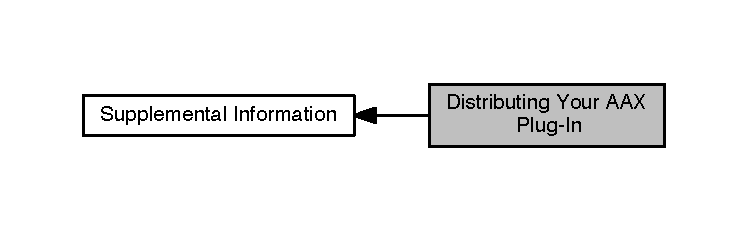
\includegraphics[width=350pt]{a00372}
\end{center}
\end{figure}
